\documentclass[t]{beamer}

% Load general definitions
% Preamble file - general definitions, package loading, etc.

%=================================
% Load packages
\usepackage{amssymb,amsmath}
\usepackage{graphicx}
\usepackage{url}
\usepackage{tikz}
\usetikzlibrary{mindmap,trees,arrows}
\usepackage{fancyvrb}
\usepackage[english]{babel}
\usepackage[latin1]{inputenc}
\usepackage{subfigure}
\usepackage{times}
\usepackage[T1]{fontenc}
\usepackage{cancel}
\usepackage{color}
\usepackage{listings}

%=================================
% Set mode
\mode<presentation>
{
	\usetheme{Madrid}
	\usecolortheme{whale}
	\useoutertheme{infolines}
	\setbeamercovered{invisible}
}

% Get rid of nav bar
\beamertemplatenavigationsymbolsempty

% Insert frame number at bottom of the page.
\usefoottemplate{\hfil\tiny{\color{black!90}\insertframenumber}} 

%=================================
% Define new commands

\newcommand\Real{{\mathbb{R}}}
%\newcommand{\vi}{\vspace{0.6\baselineskip}}
%\newcommand{\goodgap}{\hspace{\subfigtopskip}\hspace{\subfigbottomskip}}


% Equation environments
\newcommand{\beq}{\begin{equation}}
\newcommand{\eq}{\end{equation}}
\newcommand{\beqs}{\begin{equation*}}
\newcommand{\eqs}{\end{equation*}}
\newcommand{\beqn}{\begin{eqnarray}}
\newcommand{\eqn}{\end{eqnarray}}

% Bold variables
\newcommand{\mbf}[1]{\ensuremath{\mathbf{#1}}}

% Itemization
\newcommand{\bitem}{\begin{itemize}}
\newcommand{\eitem}{\end{itemize}}
\newcommand{\spitem}{\vskip 1em\item}
\newcommand{\bitems}{\begin{itemize}\item}
\newcommand{\benums}{\begin{enumerate}\item}
\newcommand{\eenum}{\end{enumerate}}

% color blocks
\newenvironment{colorblock}[2]{%
\setbeamercolor{block title}{#2}
\begin{block}{#1}}{\end{block}}

% Vertical spacing
\newcommand{\vone}{\vskip 1em}
\newcommand{\vhalf}{\vskip .5em}

% Frame environments
\newenvironment{ftst}[3][t]{%
\begin{frame}{environment=ftst,#1}
\frametitle{#2}
\framesubtitle{#3}}{\end{frame}}

\newenvironment{ftstf}[2]{
\begin{frame}[fragile,environment=ftstf]
\frametitle{#1}
\framesubtitle{#2}}{\end{frame}}

% colors
\definecolor{MyGray}{rgb}{0.5,0.5,0.5}
\definecolor{MyDBGray}{rgb}{0.1,0.1,0.4}
\definecolor{darkgreen}{rgb}{0,0.4,0}
\definecolor{black}{rgb}{0,0,0}
\def\defn#1{{\color{red} #1}}

% Footnote
\renewcommand{\thefootnote}{\alph{footnote}}

% Relaxed footnotes
\newcommand{\lfr}[1]{\let\thefootnote\relax\footnote{\tiny #1}}

% Verbatim environment - using FANCYVRB package
\DefineVerbatimEnvironment%
{rcode}{Verbatim}
{fontsize=\scriptsize}

% Verbatim environment - using LISTINGS package
%\lstnewenvironment{rcode} {\lstset{	language = R,
%									basicstyle = \scriptsize\ttfamily,
%									showspaces = false,
%									showstringspaces = false,
%									showtabs = false,
%									keywordstyle = \color{black}\bfseries,
%									commentstyle = \color{darkgreen},
%									numbers = none,
%									otherkeywords={	<-,
%													ggplot,
%													geom_boxplot,
%													facet_grid,
%													shapiro.test,
%													fligner.test,
%													glht,
%													with},
%									deletekeywords={data,
%													model,
%													residuals,
%													c,
%													axis,
%													default,
%													labels,
%													qq.text}}}%
%{}


% Specific definitions
\title[]{Design and Analysis of Experiments}
\subtitle[]{01 - What is Science}
\author[]{Felipe Campelo\\{\footnotesize http://orcslab.cpdee.ufmg.br/}}
\institute{Graduate Program in Electrical Engineering}
\date{\scriptsize Belo Horizonte\\August 2018}

\begin{document}

% cover page
\setbeamertemplate{footline}{}
\begin{frame}
\begin{flushright}

\includegraphics[width=.25\textwidth]{../figs/principal_completa3_ufmg}
\end{flushright}
  \titlepage
  \begin{tikzpicture}[remember picture,overlay]
  \node[anchor=south east,xshift=-5pt,yshift=122pt] at (current page.south east) {\tiny Version 2.12.2018b};
  \node[anchor=south west,yshift=0pt] at (current page.south west) {
\includegraphics[width=.15\textwidth]{../figs/by-nc-sa.png}};
  \end{tikzpicture}  
\end{frame}

%=====

% quotation page
  \begin{frame}[b]
		\frametitle{}
\begin{columns}[T]
\column{0.8\textwidth}
\flushright{\small ``\textit{Science and everyday life cannot\\and should not be separated.}''\\\ \\
Rosalind Franklin (1920 -- 1958)\\
English Chemist and X-ray crystallographer}
\column{0.2\textwidth}
\begin{tikzpicture}[remember picture,overlay]
\node[anchor=south east,yshift=5pt,xshift=0pt] at (current page.south east)
{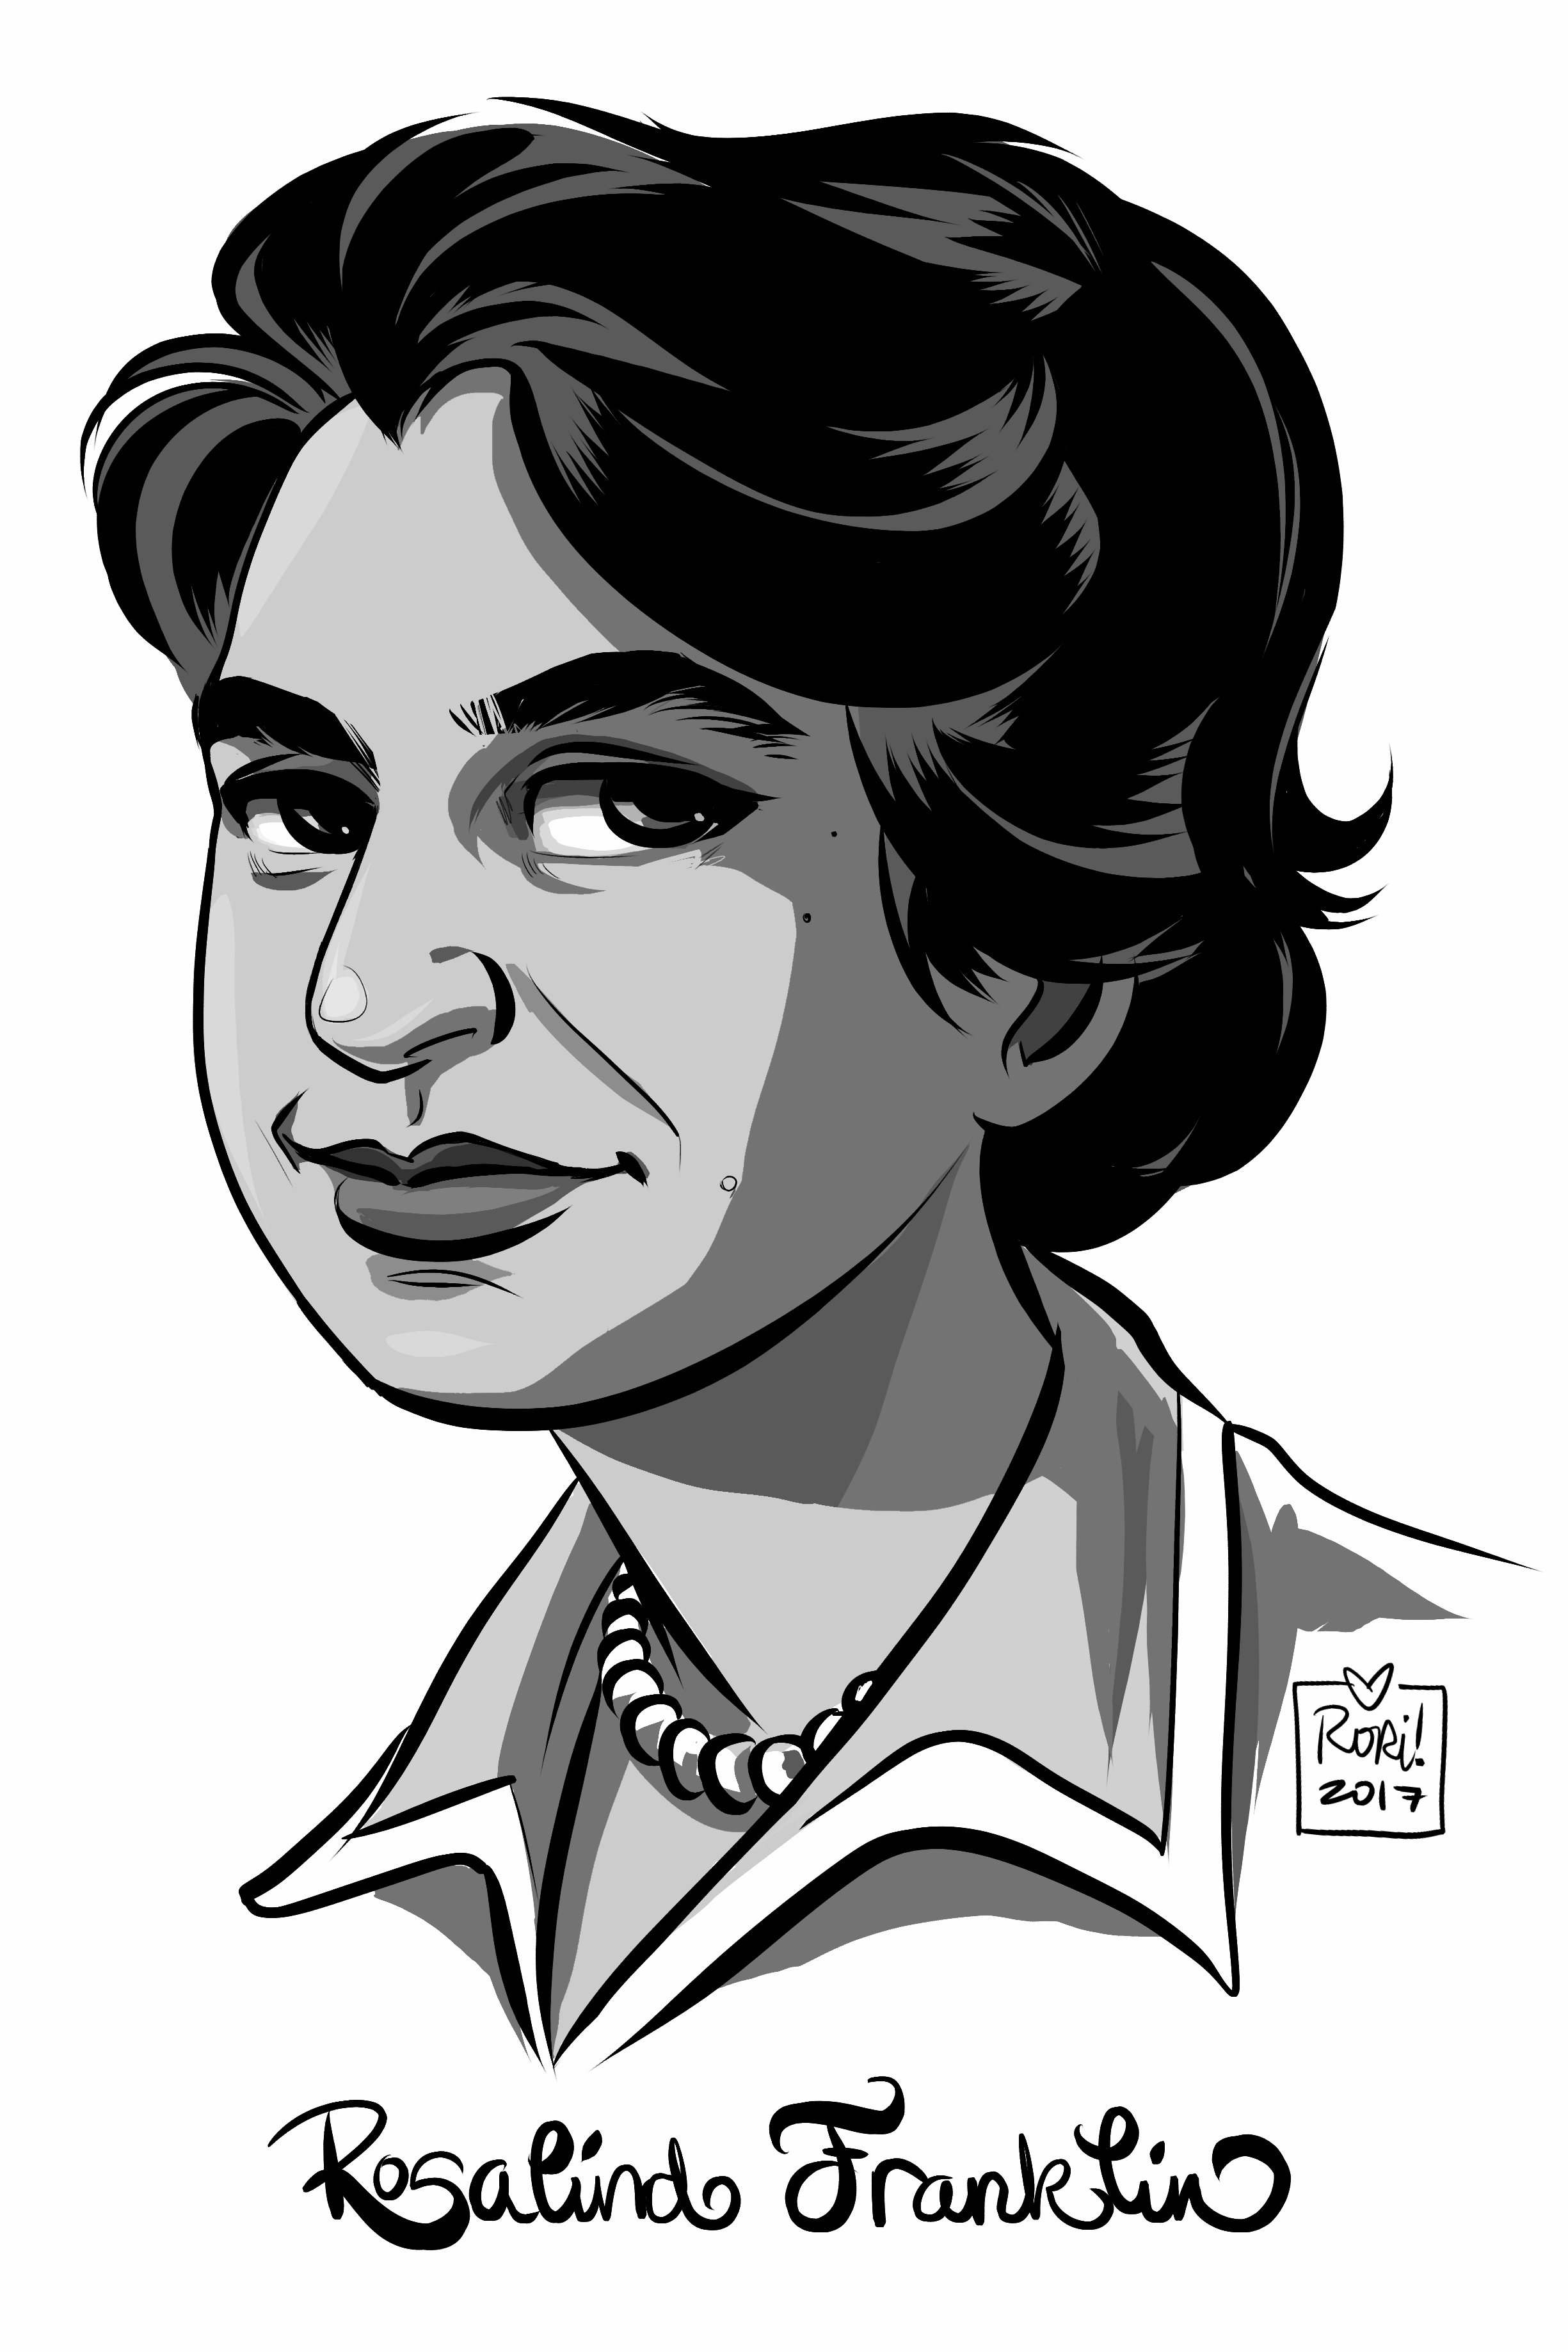
\includegraphics[width=\textwidth]{../figs/Rosalind_Franklin_CC-BY-SA.png}};
\end{tikzpicture}
\end{columns}
\vhalf
\lfr{Image: \url{https://commons.wikimedia.org/wiki/File:Rosalind_Franklin_CC-BY-SA.png}}
\end{frame}

%=====

% Main slides
\begin{ftst}
{What is science?}
{Some common misconceptions}

\bitem\item Science is a collection of facts; {\color{red}$\times$}
	\item Science is the creation of new gadgets; {\color{red}$\times$}
	\item Scientific ideas are absolute and unchangeable; {\color{red}$\times$}
	\item Scientific ideas are subject to change, therefore unreliable; {\color{red}$\times$}
	\item Observations give answers directly to the scientists; {\color{red}$\times$}
	\item Science \textbf{proves} stuff; {\color{red}$\times$}
	\item Science can only \textbf{disprove} stuff; {\color{red}$\times$}
	\item The scientist works to \textbf{show} that his/her theory is right;{\color{red}$\times$}
	\vskip .5em
	\spitem Facts \textit{vs} hypotheses \textit{vs} theories \textit{vs} laws;
\eitem
\lfr{\textbf{Essential reading}: Common Misconceptions About Science: \url{http://goo.gl/TN7k9B}}
\lfr{Image: \url{http://xkcd.com}}
\begin{tikzpicture}[remember picture,overlay]
\node[anchor=north east,yshift=-35pt,xshift=-5pt] at (current page.north east) { 
\includegraphics[height=2cm]{../figs/xkcd_science.jpg}};
\end{tikzpicture}
\end{ftst}

%=====

\begin{ftst}
{What is science?}
{A good operational definition}
\vone
\begin{columns}[T]
\column{0.3\textwidth}
\begin{tikzpicture}[remember picture,overlay]
\node[anchor=north west,yshift=-70pt,xshift=0pt] at (current page.north west)
{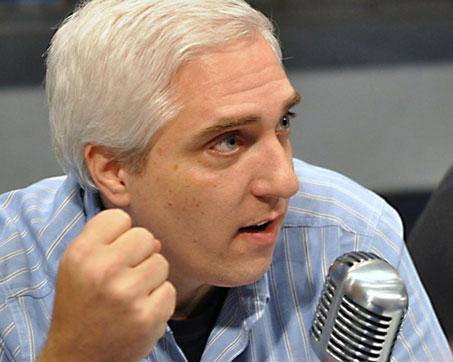
\includegraphics[width=\textwidth]{../figs/StevenNovella.jpg}};
\end{tikzpicture}
\column{0.7\textwidth}
\begin{colorblock}{}{bg=green!30,fg=black}
\flushleft{``\textit{What do you think science is?\\
There's nothing magical about science.\\
It is simply a systematic way for carefully\\
and thoroughly observing nature and\\
using consistent logic to evaluate results.}''}
\flushright{\vskip -1em -- Steven P. Novella}
\end{colorblock}
\end{columns}
\vhalf
\lfr{Image: \url{http://www.relativelyinteresting.com/definition-science-steven-novella/}}
\end{ftst}

%=====

\begin{ftst}
{What is science?}
{The scientific process}
\begin{columns}[T]
	\column{0.6\textwidth}
		\bitems Normally shown as a flowchart or a sequence of steps;
			\item Oversimplification of a complex and iterative process;
			\item Suggests an ``end'' to the process.
		\eitem
	\column{0.4\textwidth} 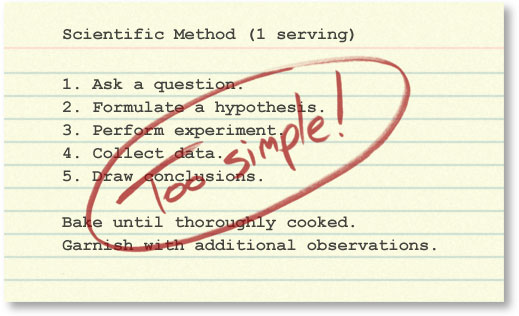
\includegraphics[width=\textwidth]{../figs/sciproc01.jpg}
\end{columns}
\vone
\begin{columns}[T]
	\column{1.02\textwidth}
		\bitems Actually includes:
			\bitems Several activities, performed at different stages;
			\item Interaction with the scientific community;
			\item Creative, ``outside the box'' thinking;
			\item Preliminary conclusions, subject to revision as new and better data become available;
			\item Learning from failures as much as from successes.
		\eitem
	\eitem
\end{columns}
\lfr{Image: \url{http://goo.gl/7cCGaz} - (c) Understanding Science, 2015. Used with permission.}
\end{ftst}

%=====

\begin{ftst}
{What is science?}
{The scientific process}
\begin{center}
	\vspace{-1.3em}
	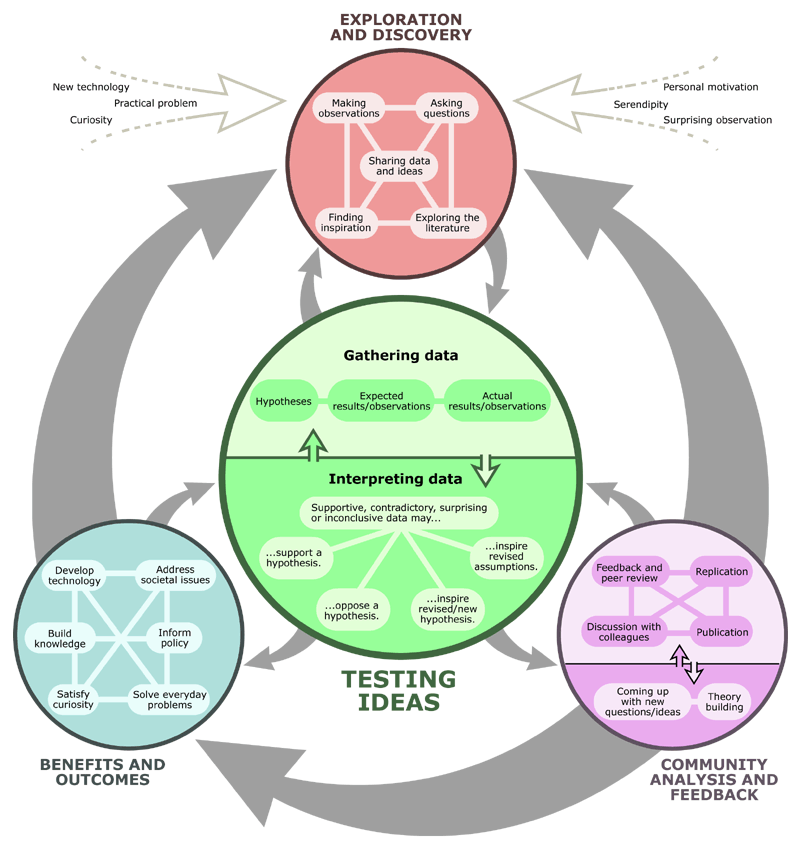
\includegraphics[width=0.56\textwidth]{../figs/sciproc02.png}
\end{center}
\lfr{Image: \url{http://goo.gl/VglXc5} - (c) Understanding Science, 2015. Used with permission.}
\end{ftst}

%=====

\begin{ftst}
{What is science?}
{The scientific process}
\vspace{-1em}
\begin{colorblock}{}{bg=green!30,fg=black}
``\textit{Dans les champs de l'observation le hasard ne favorise que les esprits pr?par?s.}'' -- \textbf{Louis Pasteur} (Univ. Lille, France, 1854).
\end{colorblock}
\vskip -0.5em
\begin{columns}[T]
\column{0.5\textwidth}
	\bitems Observations $\rightarrow$ \textbf{questions};
	\item Exploratory experimentation;
	\item Preparation + serendipity.
\eitem
\column{0.5\textwidth} 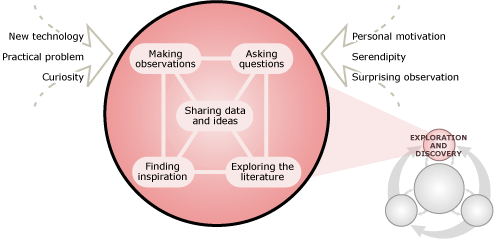
\includegraphics[width=\textwidth]{../figs/sciproc02a.png}
\end{columns}
\vhalf
\begin{columns}[T]
\column{0.3\textwidth}
\begin{block}{\footnotesize Benzene (1865)}
\centering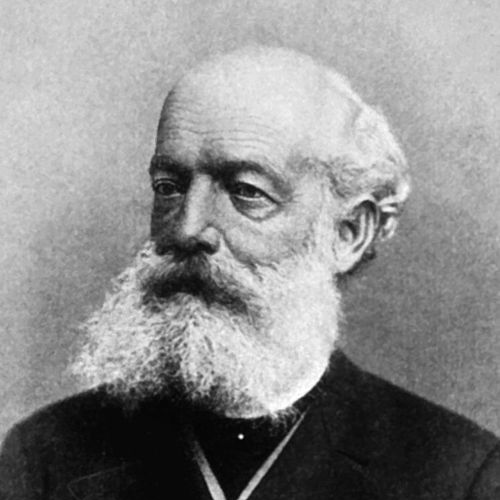
\includegraphics[width=0.35\textwidth]{../figs/kekule.png}\\
\footnotesize Kekule
\end{block}
\column{0.02\textwidth}
\column{0.3\textwidth}
\begin{block}{\footnotesize Radioactivity (1896)}
\centering
\includegraphics[width=0.35\textwidth]{../figs/becquerel.png}\\\footnotesize Becquerel
\end{block}
\column{0.02\textwidth}
\column{0.3\textwidth}
\begin{block}{\footnotesize Penicillin (1928)}
\centering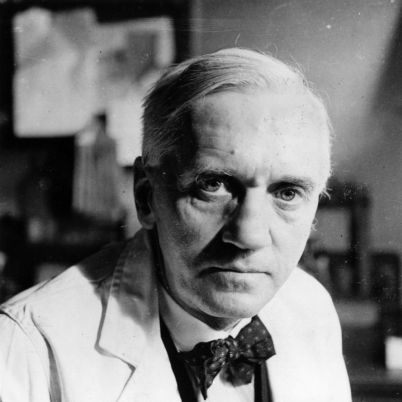
\includegraphics[width=0.35\textwidth]{../figs/fleming.png}\\\footnotesize Fleming
\end{block}
\column{0.01\textwidth}
\end{columns}
\lfr{Top image: \url{http://goo.gl/fy8Glh} - (c) Understanding Science, 2015. Used with permission.}
\lfr{Scientists: \url{http://goo.gl/SG6sgp} | \url{http://goo.gl/rhLC9C} | \url{http://goo.gl/CFj8Ml}}
\end{ftst}

%=====

\begin{ftst}
{What is science?}
{The scientific process}
\bitems Drawing and testing hypotheses;
	\item Comparing alternative explanations;
	\item Accepting / rejecting ideas based on \textbf{evidence};
	\item \textbf{Predictions} \textit{versus} \textbf{observation}: corroboration or refutation?
\eitem

\begin{tikzpicture}[remember picture,overlay]
\node[anchor=south,yshift=15, xshift=20pt] at (current page.south) {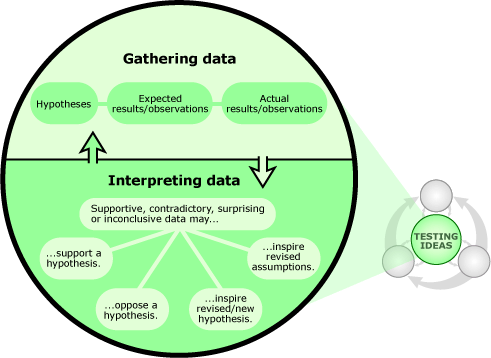
\includegraphics[width=0.55\textwidth]{../figs/sciproc02b.png}};
\end{tikzpicture}
\lfr{Image: \url{http://goo.gl/aOgSqT} - (c) Understanding Science, 2015. Used with permission.}
\end{ftst}

%=====

%\begin{ftst}
%{What is science?}
%{The scientific process}
%\vspace{-0.4em}
%\begin{columns}[T]
%\column{0.8\textwidth}
%	\textbf{James Lind} (1747):\\
%	\bitems Observation: scurvy in sailors;
%		\item Conjecture: Caused by the body rottenning;
%		\item Idea: attempt to avoid/reverse effects with acidic substances;
%	\eitem
%\column{0.2\textwidth}
%\end{columns}
%\vone
%Separation of a group of 12 affected sailors in six groups with identical diets, except for the addition of a supplement:
%\begin{columns}[T]
%\column{0.30\textwidth}
%\begin{colorblock}{Group 1}{bg=green!25,fg=black}
%	\small Cider.
%\end{colorblock}
%\begin{colorblock}{Group 4}{bg=gray!25,fg=black}
%	\small Sea water.
%\end{colorblock}
%\column{0.30\textwidth}
%\begin{colorblock}{Group 2}{bg=gray!25,fg=black}
%	\small Vitriol.
%\end{colorblock}
%\begin{colorblock}{Group 5}{bg=green!60,fg=black}
%	\small Oranges and lemons.
%\end{colorblock}
%\column{0.30\textwidth}
%\begin{colorblock}{Group 3}{bg=gray!25,fg=black}
%	\small Vinegar.
%\end{colorblock}
%\begin{colorblock}{Group 6}{bg=gray!25,fg=black}
%	\small Tea.
%\end{colorblock}
%\end{columns}
%\begin{tikzpicture}[remember picture,overlay]
%\node[anchor=north east,yshift=-40, xshift=-10pt] at (current page.north east) {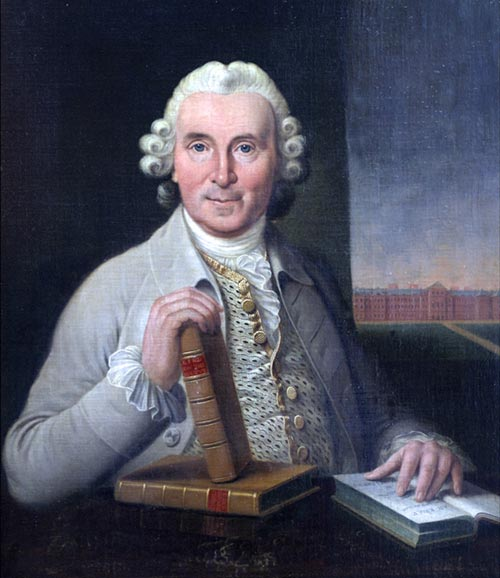
\includegraphics[width=2.2cm]{../figs/lind.jpg}};
%\end{tikzpicture}
%\lfr{Image: \url{http://commons.wikimedia.org/wiki/File:James_Lind_by_Chalmers.jpg}}
%\end{ftst}

%=====

\begin{ftst}
{What is science?}
{The scientific process}
\begin{columns}[T]
\column{0.5\textwidth}
Interaction with the scientific community is \textbf{fundamental}:

	\bitems Colleagues;
	\item Collaborators;
	\item Reviewers;
	\item Rivals;
\eitem
\column{0.5\textwidth} \vskip -1em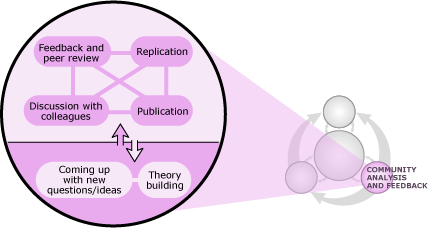
\includegraphics[width=1\textwidth]{../figs/sciproc02c.png}
\end{columns}
\vone
This interaction plays essential roles for the progress of research:
\vskip -.5em
\begin{columns}[T]
\column{0.22\textwidth}\begin{block}{Criticism}
	\centering
\includegraphics[width=\textwidth]{../figs/community2.png}
\end{block}
\column{0.22\textwidth}\begin{block}{Inspiration}
	\centering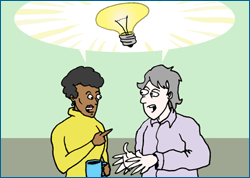
\includegraphics[width=\textwidth]{../figs/community3.png}
\end{block}
\column{0.22\textwidth}\begin{block}{Vigilance}
	\centering
\includegraphics[width=\textwidth]{../figs/community4.png}
\end{block}
\column{0.22\textwidth}\begin{block}{Motivation}
	\centering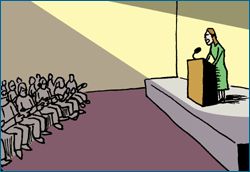
\includegraphics[width=\textwidth]{../figs/community5.png}
\end{block}
\end{columns}
\lfr{All images: \url{http://goo.gl/9pSCTG} - (c) Understanding Science, 2015. Used with permission.}
\end{ftst}

%=====

\begin{ftst}
{What is science?}
{The scientific process}
Publication and peer review.
\begin{columns}[T]
\column{0.5\textwidth}
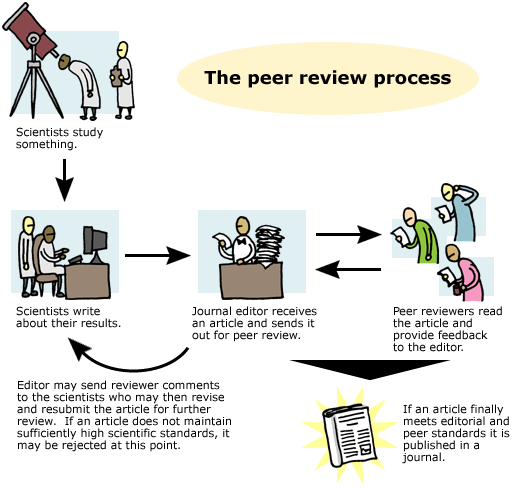
\includegraphics[width=1.15\textwidth]{../figs/peerreview.png}
\column{0.5\textwidth}
\bitems Additionally,  \textit{post-publication review} by the wider scientific community;
\spitem \textbf{Replication} and verification of results;
\spitem \textbf{Reproducibility} is essential.
\eitem
\end{columns}
\lfr{Image: \url{http://goo.gl/VWCVkK} - (c) Understanding Science, 2015. Used with permission.}
\end{ftst}

%=====

\begin{ftst}
{What is science?}
{The scientific process}
\begin{columns}[T]
\column{0.55\textwidth}
The scientific process is a way of building knowledge:
\bitems Generate and test new ideas about how the world works;
	\item Iteratively increasing the reliability of the knowledge;
\eitem
\column{0.45\textwidth}\vskip -1em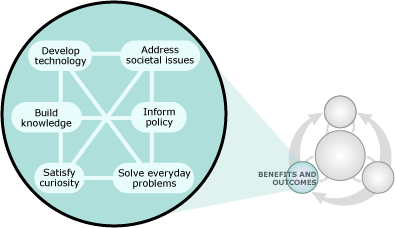
\includegraphics[width=\textwidth]{../figs/sciproc02d.png}
\end{columns}
\vhalf
\begin{columns}[T]
\column{0.32\textwidth}\begin{block}{}
		\centering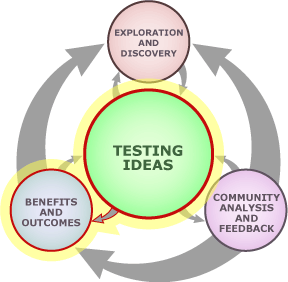
\includegraphics[width=0.85\textwidth]{../figs/benefitschart1.png}\\
		\scriptsize Knowledge$\rightarrow$Applications
	\end{block}
\column{0.32\textwidth}\begin{block}{}
		\centering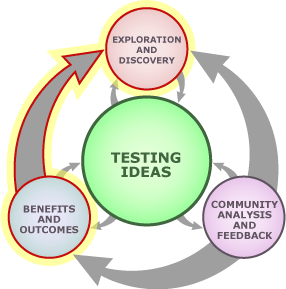
\includegraphics[width=0.83\textwidth]{../figs/benefitschart2.png}\\
		\scriptsize Technologies$\rightarrow$Discovery
	\end{block}
\column{0.32\textwidth}\begin{block}{}
		\centering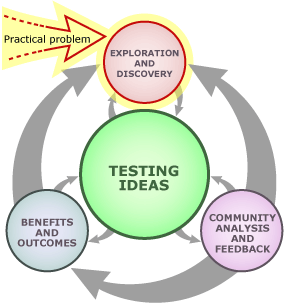
\includegraphics[width=0.79\textwidth]{../figs/benefitschart3.png}\\
		\scriptsize Applications$\rightarrow$Investigation
	\end{block}
\end{columns}
\lfr{All images: \url{http://goo.gl/IBRSoQ} - (c) Understanding Science, 2015. Used with permission.}
\end{ftst}

%=====

%\begin{ftst}
%{What is science?}
%{To wrap it up}
%\vone
%\begin{columns}[T]
%\column{0.18\textwidth}
%\begin{tikzpicture}[remember picture,overlay]
%\node[anchor=north west,yshift=-70pt,xshift=0pt] at (current page.north west)
%{
\includegraphics[width=\textwidth]{../figs/caranha.png}};
%\end{tikzpicture}
%\column{0.82\textwidth}
%\begin{colorblock}{}{bg=green!30,fg=black}
%\flushleft{``\textit{It is important to be literate in the scientific method,\\
%	not only for the sake of your own research. We are also\\
%	agents of change in the population and, as such, we\\
%	need to be aware of good and bad science, and able\\
%	to point the difference to the society.}''}
%\flushright{\vskip -1em -- Claus C. Aranha}
%\end{colorblock}
%\end{columns}
%\vhalf
%\lfr{Image: \url{http://lattes.cnpq.br/2897895256340893}}
%\end{ftst}

%=====

\begin{ftst}
{Bibliography}
{\ }
\scriptsize
\textbf{Required reading}

\benums \textit{Understanding Science}. 2014. University of California Museum of Paleontology. 3 January 2014. - 
{\tiny \url{http://www.understandingscience.org}}
	\item F.L.H. Wolfs, \textit{APPENDIX E: Introduction to the Scientific Method}. - 
	{\tiny \url{http://goo.gl/osGpU}}
\eenum

\textbf{Recommended reading}

\benums Carl Sagan,\textit{The demon-haunted world: science as a candle in the dark},\\Random House, 1996.
	\item The Skeptics Guide to the Universe. - 
	{\tiny \url{http://www.theskepticsguide.org}}
\eenum
\end{ftst}

%=====

\begin{ftstf}{About this material}{Conditions of use and referencing}
\centering\footnotesize This work is licensed under the Creative Commons CC BY-NC-SA 4.0 license\\(Attribution Non-Commercial Share Alike International License version 4.0).\\
\vhalf
\url{http://creativecommons.org/licenses/by-nc-sa/4.0/}\\
\vone
\footnotesize Please reference this work as:\\
\footnotesize \flushleft Felipe Campelo (2018), \textit{Lecture Notes on Design and Analysis of Experiments}.\\Online: {\scriptsize\url{https://github.com/fcampelo/Design-and-Analysis-of-Experiments}}\\
Version 2.12. Creative Commons BY-NC-SA 4.0.\\

\begin{Verbatim}[fontsize=\tiny]
    @Misc{Campelo2018,
      title={Lecture Notes on Design and Analysis of Experiments},
      author={Felipe Campelo},
      howPublished={\url{https://github.com/fcampelo/Design-and-Analysis-of-Experiments}},
      year={2018},
      note={Version 2.12. Creative Commons BY-NC-SA 4.0.},
    }
\end{Verbatim}

\begin{tikzpicture} [remember picture,overlay]
\node[anchor=south,yshift=0pt] at (current page.south){ \includegraphics[width=.2\textwidth]{../figs/CCSomerights.png}};
\end{tikzpicture}
\end{ftstf}


\end{document}